%%%%%%%%%%%%%%%%%%%%%%%%%%%%%%%%%%%%%%%%%%%%%%%%%%%%%%%%%

\begin{table*}[bp]
\newcolumntype{Y}{>{\raggedright\arraybackslash}X}
\newcolumntype{Z}{>{\centering\arraybackslash}X}
\centering
\footnotesize
%\small
\setlength\tabcolsep{1pt}
\renewcommand{\arraystretch}{1.2}

\begin{tabularx}{\textwidth}{l c YYY c YYY c YYY}
\toprule

 %& \multicolumn{9}{@{\hskip 0.15in}c}{Base training set: R-VQA$_{NC}$ \,+\, H-VQA$_C$ }\\
%\cmidrule[0.5pt]{2-10}

{\multirow{2}{*}{\bf Backbone}}~~~ &~~~~&
\multicolumn{3}{@{\hskip 0.11in}c}{\bf CUB} &~~~~& 
\multicolumn{3}{@{\hskip 0.11in}c}{\bf SUN} &~~~~& 
\multicolumn{3}{@{\hskip 0.11in}c}{\bf AWA2} \\

\cmidrule{3-5}\cmidrule{7-9}\cmidrule{11-13}

&& \textit{Seen} & \textit{Novel} & \textit{Harm.} 
&& \textit{Seen} & \textit{Novel} & \textit{Harm.} 
&& \textit{Seen} & \textit{Novel} & \textit{Harm.} \\

\midrule

% RN101 & \multirow{8}{*}{\rotatebox[origin=c]{45}{'This is a photo of a \{\}'}} &&
RN50 &  & 
45.90 & 45.44 & 45.67 &&
44.61 & 48.96 & 46.68 &&
87.86 & 82.48 & 85.08 \\ 

RN101 &  & 
48.86 & 49.44 & 49.15 && 
45.16 & 49.24 & 47.11 && 
88.66 & 84.79 & 86.67 \\ 

RN50x4 &  & 
51.89 & 55.27 & 53.53 && 
48.53 & 50.56 & 49.52 && 
92.09 & 86.52 & 89.22 \\ 

RN50x16 &  & 
56.82 & 55.19 & 55.99 && 
49.07 & 54.44 & 51.62 &&
94.36 & 89.11 & 91.65 \\ 

RN50x64 &  & 
63.81 & 57.19 & 60.32 && 
55.28 & 51.59 & 53.37 && 
95.11 & 90.11 & 92.54 \\ 

ViTB32 &  & 
51.35 & 49.65 & 50.49 && 
48.26 & 50.97 & 49.58 && 
90.99 & 85.69 & 88.26 \\ 

ViTB32$^{\dag}$ &   & 
61.46 & 58.09 & 59.73 && 
50.66 & 53.75 & 52.16 && 
87.84 & 82.12 & 84.88 \\

ViTB16 &  & 
55.76 & 56.23 & 55.99 &&
50.97 & 56.11 & 53.42 && 
93.68 & 87.19 & 90.32 \\ 

ViTL14 &  & 
62.62 & 63.19 & 62.90 &&
55.97 & 58.06 & 56.99 && 
95.80 & 89.39 & 92.48 \\

% ViTL14$^{\dag}$ & & 
% 64.45 & 62.13 & 63.26 && 
% 57.79 & 61.53 & 59.60 && 
% 96.06 & 88.45 & 92.10 \\

\midrule
\band
ViTL14$^{\Uparrow}$ & & 
\textbf{64.45} & \textbf{62.69} & \textbf{63.56} && 
\textbf{57.79} & \textbf{62.64} & \textbf{60.12} && 
\textbf{96.06} & \textbf{89.91} & \textbf{92.88} \\

\bottomrule
\end{tabularx}
%\vspace{-0.05in}
\caption{Results of using publicly available pre-trained CLIP\cite{CLIP} models with different backbones to evaluate three standard GSZL datasets. ${\Uparrow}$ indicates we used a set of captions similar to the proposed by OpenAI to test on Imagenet\cite{Imagenet}, ${\dag}$ indicates the model used was trained on the Laion400M\cite{LAION400M} dataset.
}
\label{tab:all_datasets_clip_only}
\vspace{-0.0in}
\end{table*}

%%%%%%%%%%%%%%%%%%%%%%%%%%%%%%%%%%%%%%%%%%%%%%%%%%%%%%%%%

% \begin{table}[!ht]
%     \centering
%     \begin{tabular}{ll>{\centering\arraybackslash}p{1.25cm}>{\centering\arraybackslash}p{1.25cm}>{\centering\arraybackslash}p{1.25cm}l}
%         \toprule
%         \multicolumn{1}{c}{Dataset} & Backbone & Seen & Unseen & Harmonic & \multicolumn{1}{c}{Caption}  \\ \hline
%         \multirow{10}{*}{OpenAI Dataset} & RN50 & 45.9 & 45.44 & 45.67 & \multirow{8}{*}{'This is a photo of a \{\}'}  \\ 
%         ~ & RN101 & 48.86 & 49.44 & 49.15 &   \\ 
%         ~ & RN50x4 & 51.89 & 55.27 & 53.53 &   \\ 
%         ~ & RN50x16 & 56.82 & 55.19 & 55.99 &   \\ 
%         ~ & RN50x64 & 63.81 & 57.19 & 60.32 &   \\ 
%         ~ & ViTB32 & 51.35 & 49.65 & 50.49 &   \\ 
%         ~ & ViTB16 & 55.76 & 56.23 & 55.99 &   \\ 
%         ~ & ViTL14 & 62.62 & 63.19 & 62.90 &   \\ \cmidrule{2-6}
%         ~ & ViTL14 & 64.45 & 62.13 & 63.26 & 'Image of a \{\}'  \\ \cmidrule{2-6}
%         \band ~ & ViTL14 & \textbf{64.45} & \textbf{62.69} & \textbf{63.56} & Prompts used for Imagenet  \\ \midrule
%         Laion400 Dataset & ViTB32 & 61.46 & 58.09 & 59.73 & 'Image of a \{\}' \\ 
%         \bottomrule
%     \end{tabular}
%     \vspace{0.01in}
%     \caption{}
%     \label{tab:clip_alone_cub}
% \end{table}


% \begin{table}[!ht]
%     \centering
%     \begin{tabular}{ll>{\centering\arraybackslash}p{1.25cm}>{\centering\arraybackslash}p{1.25cm}>{\centering\arraybackslash}p{1.25cm}l}
%         \toprule
%         \multicolumn{1}{c}{Dataset} & Backbone & Seen & Unseen & Harmonic & \multicolumn{1}{c}{Caption} \\ \hline
%         \multirow{10}{*}{OpenAI Dataset} & RN50 & 44.61 & 48.96 & 46.68 & \multirow{8}{*}{'This is a photo of a \{\}'} \\ 
%         ~ & RN101 & 45.16 & 49.24 & 47.11 & ~ \\ 
%         ~ & RN50x4 & 48.53 & 50.56 & 49.52 & ~ \\ 
%         ~ & RN50x16 & 49.07 & 54.44 & 51.62 & ~ \\ 
%         ~ & RN50x64 & 55.28 & 51.59 & 53.37 & ~ \\ 
%         ~ & ViTB32 & 48.26 & 50.97 & 49.58 & ~ \\ 
%         ~ & ViTB16 & 50.97 & 56.11 & 53.42 & ~ \\ 
%         ~ & ViTL14 & 55.97 & 58.06 & 56.99 & ~ \\ \cmidrule{2-6}
%         ~ & ViTL14 & 57.79 & 61.53 & 59.60 &  'Image of a \{\}' \\ \cmidrule{2-6}
%         \band ~ & ViTL14 & \textbf{57.79} & \textbf{62.64} & \textbf{60.12} & Prompts used for Imagenet \\ \midrule
%         laion400 Dataset & ViTB32 & 50.66 & 53.75 & 52.16 &  'Image of a \{\}' \\ 
%         \bottomrule
%     \end{tabular}
%     \vspace{0.01in}
%     \caption{Results of using publicly available pre-trained CLIP models with different backbones with the SUN dataset in the standard GSZL test splits.}
%     \label{tab:clip_alone_sun}
% \end{table}

% \begin{table}[!ht]
%     \newcolumntype{Y}{>{\raggedright\arraybackslash}X}
%     \newcolumntype{Z}{>{\centering\arraybackslash}X}
%     \centering
%     \footnotesize
%     %\small
%     \setlength\tabcolsep{1pt}
%     \renewcommand{\arraystretch}{1.2}

%     \begin{tabular}{ll>{\centering\arraybackslash}p{1.25cm}>{\centering\arraybackslash}p{1.25cm}>{\centering\arraybackslash}p{1.25cm}l}
%         \toprule
%         \multicolumn{1}{c}{Dataset} & Backbone & Seen & Unseen & Harmonic & \multicolumn{1}{c}{Caption} \\ \hline
%         \multirow{10}{*}{OpenAI Dataset} & RN50 & 87.86 & 82.48 & 85.08 & \multirow{8}{*}{'This is a photo of a \{\}'} \\ 
%         ~ & RN101 & 96.06 & 89.91 & 92.88 & ~ \\ 
%         ~ & RN50x4 & 92.09 & 86.52 & 89.22 & ~ \\ 
%         ~ & RN50x16 & 96.06 & 89.91 & 92.88 & ~ \\ 
%         ~ & RN50x64 & 95.11 & 90.11 & 92.54 & ~ \\ 
%         ~ & ViTB32 & 90.99 & 85.69 & 88.26 & ~ \\ 
%         ~ & ViTB16 & 93.68 & 87.19 & 90.32 & ~ \\ 
%         ~ & ViTL14 & 95.80 & 89.39 & 92.48 & ~ \\ \cmidrule{2-6}
%         ~ & ViTL14 & 96.06 & 88.45 & 92.10 &  'Image of a \{\}' \\ \cmidrule{2-6}
%         \band ~ & ViTL14 & \textbf{96.06} & \textbf{89.91} & \textbf{92.88} & Prompts used for Imagenet \\ \midrule
%         laion400 Dataset & ViTB32 & 87.84 & 82.12 & 84.88 &  'Image of a \{\}' \\ 
%         \bottomrule
%     \end{tabular}
%     \vspace{0.01in}
%     \caption{Results of using publicly available pre-trained CLIP models with different backbones with the AWA2 dataset in the standard GSZL test splits.}
%     \label{tab:clip_alone_awa2}
% \end{table}



% ==========================================================================
% ==========================================================================




% ==========================================================================
% ==========================================================================



\begin{table*}[bp] % [hbt!]
\newcolumntype{Y}{>{\raggedright\arraybackslash}X}
\newcolumntype{Z}{>{\centering\arraybackslash}X}
\centering
\footnotesize
\setlength\tabcolsep{1pt}
\renewcommand{\arraystretch}{1.2}

\begin{tabularx}{\textwidth}{cl c YYY c YYY c YYY c YYY c YYY}
\toprule

% \multicolumn{21}{@{\hskip 0.11in}c}{\bf \shortstack{GZSL Methods using CLIP Features\\ CUB Dataset}}  \\
\multicolumn{22}{@{\hskip 0.11in}c}{\bf GZSL Methods using CLIP Visual Features} \\
\midrule

{\multirow{2}{*}{\bf \shortstack{Data \\set }}} &
{\multirow{2}{*}{\bf \shortstack{Back \\bone }}} &
% {\multirow{2}{*}{\bf \shortstack{Data~~~~ | Back \\set~~~~~~~ | bone }}} &~&
\multicolumn{3}{@{\hskip 0.11in}c}{\bf tfVAEGAN} &~~& 
\multicolumn{3}{@{\hskip 0.11in}c}{\bf CADA-VAE} &~~& 
\multicolumn{3}{@{\hskip 0.11in}c}{\bf SDGZSL} &~~& 
\multicolumn{3}{@{\hskip 0.11in}c}{\bf FREE} &~~& 
\multicolumn{3}{@{\hskip 0.11in}c}{\bf CE} \\


% \cmidrule{3-5}\cmidrule{7-9}\cmidrule{11-13}\cmidrule{15-17}\cmidrule{19-21}
\cmidrule{4-6}\cmidrule{8-10}\cmidrule{12-14}\cmidrule{16-18}\cmidrule{20-22}

&&& \textit{Seen} & \textit{Novel} & \textit{Harm.} 
&& \textit{Seen} & \textit{Novel} & \textit{Harm.} 
&& \textit{Seen} & \textit{Novel} & \textit{Harm.} 
&& \textit{Seen} & \textit{Novel} & \textit{Harm.} 
&& \textit{Seen} & \textit{Novel} & \textit{Harm.} \\

\midrule
% \multicolumn{21}{@{\hskip 0.11in}c}{\bf CUB Dataset} \\
% \midrule

% &{R50} &  & 
% 66.91 & 49.96 & 57.20  & ~ &
% 61.67 & 56.67 & 59.06  & ~ &
% 61.24 & 56.89 & 58.98  & ~ &
% 62.95 & 47.70 & 54.28  & ~ &
% 40.72 & 37.32 & 38.95  \\

% &{R101} &  & 
% 65.83 & 60.13 & 62.85  & ~ &
% 62.31 & 61.97 & 62.14  & ~ &
% 65.03 & 59.53 & 62.16  & ~ &
% 59.41 & 60.05 & 59.73  & ~ &
% 60.00 & 52.52 & 56.01  \\

% &{R50$_{\text{x4}}$} &  & 
% 70.48 & 65.41 & 67.85  & ~ &
% 67.90 & 68.84 & 68.37  & ~ &
% 66.38 & 67.77 & 67.07  & ~ &
% 68.55 & 59.75 & 63.85  & ~ &
% 62.57 & 44.50 & 52.01 \\

% &{R50$_{\text{x16}}$} &  & 
% 73.94 & 69.22 & 71.50  & ~ &
% 76.40 & 67.15 & 71.47  & ~ &
% 72.65 & 68.92 & 70.74  & ~ &
% 71.02 & 63.27 & 66.92  & ~ &
% 61.04 & 46.26 & 52.63  \\

\parbox[t]{1mm}{\multirow{5}{*}{\rotatebox[origin=c]{90}{CUB}}}
& {R50$_{\text{x64}}$} &  & 
82.09 & 67.93 & 74.34  & ~ &
75.91 & 70.84 & 73.29  & ~ & 
74.77 & 73.70 & 74.23  & ~ &
68.53 & \underline{73.47} & 70.91  & ~ &
59.06 & 49.52 & 53.87  \\

% &{ViT$_{\text{B32}}$} &  & 
% % 64.37 & 62.08 & 63.20  & ~ &
% % 64.34 & 57.52 & 60.74  & ~ &
% % 64.20 & 59.66 & 61.84  & ~ &
% % 61.51 & 54.87 & 58.00  & ~ &
% % 60.96 & 50.55 & 55.27  \\

% &{ViT$_{\text{B16}}$} &  & 
% % 76.48 & 66.32 & 71.04  & ~ &
% % 71.13 & 67.79 & 69.42  & ~ &
% % 64.81 & \underline{74.25} & 69.21  & ~ &
% % 68.46 & 65.99 & 67.20  & ~ &
% % 58.30 & \underline{62.17} & \underline{60.17}  \\

&{ViT$_{\text{L14}}$} &  & 
\underline{77.67} & \underline{72.36} & \underline{74.92}  & ~ &
\underline{77.90} & \underline{72.98} & \underline{75.36}  & ~ &
\underline{79.50} & 73.49 & \underline{76.38}  & ~ &
\underline{79.05} & 65.38 & \underline{71.56}  & ~ &
\underline{74.04} & 46.38 & 57.03  \\

\arrayrulecolor{gray!48} \cmidrule{2-22} % \midrule
\arrayrulecolor{black}

&{ViT$_{\text{L14}}^\dag$} &  & 
80.39 & 72.86 & 76.44  & ~ &
\textbf{81.96} & 71.24 & 76.22  & ~ & 
79.19 & 74.70 & 76.88  & ~ &
78.87 & 65.89 & 71.80  & ~ &
71.49 & 48.62 & 57.88  \\

&{ViT$_{\text{L14}}^\ddag$} &  & 
80.73 & \textbf{73.59} & 76.99  & ~ &
79.51 & 74.68 & 77.01  & ~ &
\textbf{80.40} & 74.33 & 77.25  & ~ &
79.47 & \textbf{68.25} & 73.44  & ~ &
\textbf{75.12} & 51.14 & 60.86 \\

% \band
&\cellcolor{gray!18} {ViT$_{\text{L14}}^\S$} & \cellcolor{gray!18}  & 
\cellcolor{gray!18} \textbf{82.82} & \cellcolor{gray!18} 72.27 & \cellcolor{gray!18} \textbf{77.18}  & \cellcolor{gray!18} ~ &
\cellcolor{gray!18} 81.47 & \cellcolor{gray!18} \textbf{75.05} & \cellcolor{gray!18} \textbf{78.13}  & \cellcolor{gray!18} ~ &
\cellcolor{gray!18} 80.38 & \cellcolor{gray!18} \textbf{75.67} & \cellcolor{gray!18} \textbf{77.96}  & \cellcolor{gray!18} ~ &
\cellcolor{gray!18} \textbf{80.48} & \cellcolor{gray!18} 67.54 & \cellcolor{gray!18} \textbf{73.45}  & \cellcolor{gray!18} ~ &
\cellcolor{gray!18} 71.15 & \cellcolor{gray!18} \textbf{56.82} & \cellcolor{gray!18} \textbf{63.18} \\

% ===============
% ===============

\midrule
% \multicolumn{21}{@{\hskip 0.11in}c}{\bf SUN Dataset} \\
% \midrule

% &{R50} &  & 
% % 51.94 & 53.40 & 52.66  & ~ &
% % 47.87 & 61.88 & 53.98  & ~ &
% % 43.29 & 54.10 & 48.10  & ~ &
% % 53.10 & 54.24 & 53.66  & ~ &
% % 38.84 & 52.85 & 44.77  \\

% &{R101} &  & 
% % 54.53 & 62.99 & 58.46  & ~ &
% % 53.02 & 61.53 & 56.96  & ~ &
% % 53.88 & 63.96 & 58.49  & ~ &
% % 53.18 & 58.19 & 55.57  & ~ &
% % 51.24 & 55.83 & 53.44  \\

% &{R50$_{\text{x4}}$} &  & 
% % 54.38 & 65.00 & 59.22  & ~ &
% % 55.16 & 60.56 & 57.73  & ~ &
% % 55.00 & 65.62 & 59.84  & ~ &
% % 53.37 & 62.57 & 57.61  & ~ &
% % 54.92 & 55.07 & 55.00  \\

% &{R50$_{\text{x16}}$} &  & 
% % 57.87 & 68.33 & 62.67  & ~ &
% % 57.64 & 62.92 & 60.16  & ~ &
% % 46.71 & 61.18 & 52.97  & ~ &
% % 54.22 & 62.22 & 57.95  & ~ &
% % 54.26 & \underline{60.21} & 57.08  \\

\parbox[t]{1mm}{\multirow{5}{*}{\rotatebox[origin=c]{90}{SUN}}}
&{R50$_{\text{x64}}$} &  & 
57.21 & \underline{69.79} & 62.88  & ~ &
59.46 & 65.63 & 62.39  & ~ &
57.17 & 66.60 & 61.52  & ~ &
\underline{60.04} & 57.78 & 58.89  & ~ &
50.04 & 59.10 & 54.19  \\

% &{ViT$_{\text{B32}}$} &  & 
% % 58.14 & 63.40 & 60.66  & ~ &
% % 54.50 & 61.94 & 57.98  & ~ &
% % 56.43 & 61.67 & 58.93  & ~ &
% % 51.67 & 61.11 & 55.99  & ~ &
% % 53.95 & 52.92 & 53.43  \\

% &{ViT$_{\text{B16}}$} &  & 
% % 57.98 & 67.01 & 62.17  & ~ &
% % 54.69 & 62.08 & 58.15  & ~ &
% % 57.40 & \underline{66.94} & 61.81  & ~ &
% % 54.38 & 59.93 & 57.02  & ~ &
% % 55.12 & 56.94 & 56.02  \\

&{ViT$_{\text{L14}}$} &  & 
\underline{59.84} & 68.89 & \underline{64.05}  & ~ &
\underline{62.11} & \underline{63.40} & \underline{63.18}  & ~ &
\underline{63.57} & 62.71 & \underline{63.13}  & ~ &
58.18 & \underline{62.71} & \underline{60.36}  & ~ &
\underline{60.16} & 57.85 & \underline{58.98}  \\

\arrayrulecolor{gray!48} \cmidrule{2-22}
\arrayrulecolor{black}

&{ViT$_{\text{L14}}^\dag$} &  & 
61.75 & \textbf{70.49} & 65.83  &\cellcolor{gray!18}  ~ &
\cellcolor{gray!18} \textbf{61.47} &\cellcolor{gray!18}  65.76 &\cellcolor{gray!18}  \textbf{63.54}  & ~ &
\textbf{62.56} & 64.44 & 63.49  & ~ &
\textbf{58.95} & 62.99 & 60.90  & ~ &
52.79 & \textbf{64.37} & 58.01  \\

&{ViT$_{\text{L14}}^\ddag$} &  & 
60.93 & 67.08 & 63.86  & ~ &
57.95 & \textbf{68.19} & 62.65  & ~ &
60.08 & 67.15 & 63.42  & ~ &
58.37 & 62.43 & 60.33  & ~ &
56.78 & 64.03 & 60.19  \\

&{ViT$_{\text{L14}}^\S$} &\cellcolor{gray!18}  & 
\cellcolor{gray!18} \textbf{62.25} &\cellcolor{gray!18}  70.03 &\cellcolor{gray!18}  \textbf{65.91}  & ~ &
58.91 & 66.74 & 62.58  &\cellcolor{gray!18}  ~ &
\cellcolor{gray!18} 60.70 &\cellcolor{gray!18}  \textbf{67.50} &\cellcolor{gray!18}  \textbf{63.92}  &\cellcolor{gray!18}  ~ &
\cellcolor{gray!18} 58.72 &\cellcolor{gray!18}  \textbf{63.61} &\cellcolor{gray!18}  \textbf{61.07}  &\cellcolor{gray!18}  ~ &
\cellcolor{gray!18} \textbf{59.65} &\cellcolor{gray!18}  60.90 &\cellcolor{gray!18}  \textbf{60.27}  \\

% ===============
% ===============

\midrule
% \multicolumn{21}{@{\hskip 0.11in}c}{\bf SUN Dataset} \\
% \midrule

% &{R50} &  & 
% % 72.02 & 60.31 & 65.65  & ~ &
% % 80.99 & 61.30 & 71.14  & ~ &
% % 77.72 & 57.66 & 66.21  & ~ &
% % 80.03 & 55.17 & 65.31  & ~ &
% % 78.84 & 45.19 & 57.45  \\

% &{R101} &  & 
% % 71.94 & 64.79 & 68.18  & ~ &
% % 85.25 & 59.34 & 70.87  & ~ &
% % 80.29 & 68.78 & 74.09  & ~ &
% % 78.64 & 59.11 & 67.49  & ~ &
% % 76.61 & 62.34 & 68.74  \\

% &{R50$_{\text{x4}}$} &  & 
% % 83.93 & \underline{68.02} & 75.15  & ~ &
% % 80.71 & \underline{69.87} & 77.02  & ~ &
% % 82.23 & 68.39 & 74.67  & ~ &
% % 83.30 & 57.29 & 67.89  & ~ &
% % 81.46 & 61.03 & 69.78  \\

% &{R50$_{\text{x16}}$} &  & 
% % 86.48 & 66.49 & 75.18  & ~ &
% % 89.35 & 65.88 & 77.30  & ~ &
% % 84.24 & \underline{73.18} & \underline{78.32}  & ~ &
% % 83.09 & 60.13 & 69.77  & ~ &
% 83.13 & 66.83 & 74.09  \\

\parbox[t]{1mm}{\multirow{5}{*}{\rotatebox[origin=c]{90}{AWA2}}}
&{R50$_{\text{x64}}$} &  & 
89.69 & 68.21 & 77.49  & ~ &
90.54 & 63.75 & 75.81  & ~ &
78.67 & 69.07 & 73.56  & ~ &
\underline{87.60} & 61.04 & 71.95  & ~ &
89.95 & 63.33 & 74.33  \\

% &{ViT$_{\text{B32}}$} &  & 
% % 84.24 & 62.41 & 71.70  & ~ &
% % 80.53 & 65.35 & 73.90  & ~ &
% % 84.33 & 62.43 & 71.75  & ~ &
% % 74.01 & 57.13 & 64.48  & ~ &
% % 78.91 & 62.86 & 69.98  \\

% &{ViT$_{\text{B16}}$} &  & 
% % 87.80 & 66.56 & 75.72  & ~ &
% % 90.56 & 65.44 & 75.80  & ~ &
% % 86.87 & 66.59 & 75.39  & ~ &
% % 77.05 & 61.58 & 68.45  & ~ &
% % 84.02 & 66.92 & 74.50  \\

&{ViT$_{\text{L14}}$} &  & 
\underline{90.95} & 69.50 & \underline{78.70}  & ~ &
\underline{92.68} & 68.14 & \underline{77.99}  & ~ &
\underline{89.99} & 68.76 & 77.91  & ~ &
81.10 & \underline{65.99} & \underline{72.77}  & ~ &
\underline{85.63} & \underline{71.96} & \underline{78.20}  \\

\arrayrulecolor{gray!48} \cmidrule{2-22}
\arrayrulecolor{black}

&{ViT$_{\text{L14}}^\dag$} &  & 
91.25 & 67.77 & 77.77  & ~ &
90.48 & 70.07 & 78.98  & ~ &
89.18 & 71.40 & 79.30  &\cellcolor{gray!18} ~ &
\cellcolor{gray!18}81.27 &\cellcolor{gray!18} \textbf{71.56} &\cellcolor{gray!18} \textbf{75.94}  &\cellcolor{gray!18} ~ &
\cellcolor{gray!18}85.12 &\cellcolor{gray!18} \textbf{78.02} &\cellcolor{gray!18} \textbf{81.41}  \\

&{ViT$_{\text{L14}}^\ddag$} &\cellcolor{gray!18}  & 
\cellcolor{gray!18}\textbf{93.40} &\cellcolor{gray!18} 72.61 &\cellcolor{gray!18} \textbf{81.70}  &\cellcolor{gray!18} ~ &
\cellcolor{gray!18}\textbf{93.51} &\cellcolor{gray!18} \textbf{73.85} &\cellcolor{gray!18} \textbf{82.53}  &\cellcolor{gray!18} ~ &
\cellcolor{gray!18}85.77 &\cellcolor{gray!18} \textbf{74.16} &\cellcolor{gray!18} \textbf{79.54}  & ~ &
81.29 & 65.62 & 72.62  & ~ &
89.85 & 64.12 & 74.84  \\

&{ViT$_{\text{L14}}^\S$} &  & 
89.62 & \textbf{73.56} & 80.80  & ~ &
93.35 & 68.14 & 78.78  &\cellcolor{gray!18} ~ &
\cellcolor{gray!18}\textbf{91.50} &\cellcolor{gray!18} 70.33 &\cellcolor{gray!18} \textbf{79.54}  & ~ &
\textbf{81.53} & 69.84 & 75.23  & ~ &
\textbf{90.78} & 67.96 & 77.73  \\

\bottomrule
\end{tabularx}
%\vspace{-0.05in}
\caption{Results of Generative and Disentanglement Based Methods for the CUB, SUN and AWA2 datasets using different features extracted from different size and architecture of the visual head from diverse CLIP models (i.e., Resnet50 (R50) and Vision Transformer (ViT)). The three bottom rows per section correspond to fine-tuned features using sentences with: $\dag$ the class names, $\ddag$ the attributes, and $\S$ both class names and attributes. The bold numbers correspond to the highest scores per column, the underline numbers correspond to the to the highest scores using features not fine-tuned, and the shaded rows correspond to the most performant image feature per method over all.}
\label{tab:gzsl_using_clip_features}
% \vspace{-0.05in}
\end{table*}

\section{Results using Unimodal Feature Extractors}
\label{sec:results_unimodal}

We evaluate all GZSL methods trained with feature extractors pre-trained using ImageNet-1k. In Figure~\ref{fig:model_backbone_size_vs_method}, we show the Harmonic Mean performance of different methods when using a specific model to extract the features of image samples. Surprisingly, CADA-VAE~\cite{CADA_VAE} and tfVAEGAN~\cite{tfvaegan} consistently outperform all methods. While current disentanglement methods show significant improvements when using features from transformer-based architectures, they are outperformed by the generative-based methods.
% From Figure~\ref{fig:model_backbone_size_vs_method}, 
We can also observe that DINO~\cite{DINO} provides better
feature representations for all methods across all datasets.


We also want to evaluate the impact of using a feature extractor with the \textit{same architecture type but trained with different learning objectives}. In Figure~\ref{fig:model_backbone_diff_objectives}, we show the Harmonic Mean performance of
different GZSL methods when using a Resnet model architecture pre-trained on Imagenet-1k as the image feature extractor. Surprisingly, the features extracted from DINO~\cite{DINO} increase the Harmonic Mean performance up to 15\% in both fine-grained datasets (i.e., CUB and SUN datasets). More surprisingly, the feature vectors extracted from MOCO perform worse than traditional supervised learning models trained with a cross-entropy objective function. MOCO's training objective is formulated by the InfoNCE loss, which encourages the model to maximize the Mutual Information (MI) between $N$ random samples containing one positive sample, and minimize the Mutual information between the anchor sample and $N-1$ negative samples. 
On the other hand, in DINO, a teacher and a student model are trained by feeding two different random transformations of an input image to each network; the objective is to maximize the similarity between both outputs, which is encouraged and measured with a cross-entropy loss. 
Thus, the generalization capabilities shown with DINO support prior observations when using its image features in classification tasks with respect to other self-supervised techniques~\cite{DINO}.


We then evaluate the impact of using feature extractors that were pre-trained with more data variety and size and summarize our findings in Figure~\ref{fig:model_backbone_data_size}. Surprisingly, features extracted from backbones trained with more data (Imagenet-21k) do not always perform better, but features extracted from bigger architectures seem consistently better. 


We show more detailed results on CUB, SUN and AWA2 using GZSL methods grouped in their corresponding families in the following subsections.
Please refer to the Appendix to check the full list of numerical results for all uni-modal backbones and GZSL methods. 

 % \vspace{0.02in}
\subsection{Results of \textbf{Embedding}-based Methods}

The ViT$_{\text{huge}}$ features pre-trained on ImageNet-21k seem to be the best for all the methods using ALE. 
However, for the AWA2 dataset, all methods perform better using the features extracted from a network pre-trained using ImageNet-1k.
For CUB and SUN datasets, the performance gap against the features extracted from a network trained using ImageNet-1k and ImageNet-21k is not significant for all methods.
More detailed results are available in Tables~\ref{tab:cub_embedding_CNN}, \ref{tab:sun_embedding_CNN} and \ref{tab:awa2_embedding_CNN} from Section~\ref{sec:all_tables} in the Appendix. 

 
% \vspace{0.02in}
\subsection{Results of \textbf{Generative}-based Methods} 

The most performant visual features are extracted from a ViT$_{\text{huge}}$ pretrained on ImageNet-21k and fine-tuned with the seen classes, using the CADA-VAE method. More interestingly, the features from a ViT$_{\text{large}}$ pretrained on ImageNet-1k seem competitive with the features from a ViT$_{\text{large}}$ pretrained on ImageNet-21k for the CE and tfVAEGAN methods respectively.
% We show results in Table~\ref{tab:subset_generative_based} when using embedding based GZSL methods. 
More detailed results are available in Tables~\ref{tab:cub_generative_CNN}, \ref{tab:sun_generative_CNN} and \ref{tab:awa2_generative_CNN} from Section~\ref{sec:all_tables} in the Appendix. 

% \begin{table*}[ht!]
\newcolumntype{Y}{>{\raggedright\arraybackslash}X}
\newcolumntype{Z}{>{\centering\arraybackslash}X}
\centering
\footnotesize
\setlength\tabcolsep{1pt}
\renewcommand{\arraystretch}{1.2}

\scalebox{0.90}{

\begin{tabularx}{\textwidth}{l c l c l c YYY c YYY c YYY}
\toprule

\multicolumn{17}{@{\hskip 0.11in}c}{\bf {CUB Dataset}}  \\ 
\midrule

{\multirow{2}{*}{\bf \shortstack{Dataset\\Pret. on}}}~ &~~~~&
{\multirow{2}{*}{\bf \shortstack{Arch\\ Type}}}~ &~~~~&
{\multirow{2}{*}{\bf Backbone}}~ &~~~~&
\multicolumn{3}{@{\hskip 0.11in}c}{\bf tfVAEGAN} &~~~~& 
\multicolumn{3}{@{\hskip 0.11in}c}{\bf CADA-VAE} &~~~~& 
\multicolumn{3}{@{\hskip 0.11in}c}{\bf CE} \\

\cmidrule{7-9}\cmidrule{11-13}\cmidrule{15-17}

&& && && \textit{Seen} & \textit{Novel} & \textit{Harm.} 
&& \textit{Seen} & \textit{Novel} & \textit{Harm.} 
&& \textit{Seen} & \textit{Novel} & \textit{Harm.} \\

\midrule

\multirow{3}{*}{I-1k} & &
\multirow{2}{*}{CNN} & &


RN101 &&
57.08 & 42.88 & 48.97 &&
58.27 & 49.71 & 53.65  &&
60.09 & \textbf{49.05} & 54.01  \\ 

&& &&\cellcolor{gray!18}RN101+FT &\cellcolor{gray!18}&
72.44 & 53.66 & 61.65 &&
76.45 & 57.53 & 65.65  &&
\cellcolor{gray!18}\textbf{76.71} &\cellcolor{gray!18} 48.81 &\cellcolor{gray!18} \textbf{59.66}  \\  

% && &&GoogleNet &&
% 38.54 & 33.34 & 35.76 &&
% 33.84 & 30.20 & 31.92  &&
% 33.72 & 26.05 & 29.39  \\ 

&& &&RN152 &&
50.23 & 44.48 & 47.18 &&
47.58 & 41.64 & 44.41  &&
45.77 & 35.52 & 40.00  \\ 

\cmidrule{3-17}

&& \multirow{1}{*}{ViT} &&ViT$_{\text{large}}$&&
\textbf{80.34} & 54.34 & 64.83 &&
61.23 & 53.31 & 56.99  &&
70.22 & 43.07 & 53.39  \\

&& &&DeiT$_{\text{base}}$ && 
73.29 & 49.44 & 59.05 &&
60.39 & 50.05 & 54.74  &&
55.68 & 38.68 & 45.65  \\  

&& &&ViTB16-DINO$^{\dag}$&& 
76.82 & 57.94 & 66.06 &&
71.95 & 55.37 & 62.58  &&
61.29 & 45.47 & 52.21  \\

\midrule

\multirow{2}{*}{I-21k} && \multirow{2}{*}{ViT} &&
ViT$_{\text{large}}$ & &
76.95 & 61.56 & 68.40 &&
72.54 & 58.94 & 65.04  &&
67.16 & 46.94 & 55.26  \\ 

% \multirow{2}{*}{I-21k} && \multirow{2}{*}{ViT} && ViT$_{\text{huge}}$ & &
% 75.15 & 62.76 & 68.40 &&
% 70.53 & 60.50 & 65.13  &&
% 49.37 & 43.76 & 46.40  \\

&& &&\cellcolor{gray!18} ViT$_{\text{huge}}$+FT &\cellcolor{gray!18} &
\cellcolor{gray!18}78.32 &\cellcolor{gray!18} \textbf{76.26} &\cellcolor{gray!18} \textbf{77.27} &\cellcolor{gray!18}&
\cellcolor{gray!18}\textbf{77.99} &\cellcolor{gray!18} \textbf{74.46} &\cellcolor{gray!18} \textbf{76.18}  &&
70.87&	44.66 &	54.79 \\

%%%%%%%%%%%%%%%%%%%%%%%%%%%%%%%%%%%%%%%%%%%%%%%%%%%%%%%%%%%%%%%%%
%%%%%%%%%%%%%%%%%%%%%%%%%%%%%%%%%%%%%%%%%%%%%%%%%%%%%%%%%%%%%%%%%

\midrule
\multicolumn{17}{@{\hskip 0.11in}c}{\bf {SUN Dataset}}  \\ 
\midrule

\multirow{3}{*}{I-1k} & &
\multirow{2}{*}{CNN} & &

\cellcolor{gray!18}RN101 &\cellcolor{gray!18}&
38.95 & 45.62 & 42.03  & ~ &
34.15 & 48.96 & 40.23  &\cellcolor{gray!18} ~ &
\cellcolor{gray!18}51.24 &\cellcolor{gray!18} \textbf{55.83} &\cellcolor{gray!18} \textbf{53.44}  \\ 

&& &&RN101+FT &&
35.08 & 38.06 & 36.51  & ~ &
39.84 & 51.60 & 44.97  & ~ &
29.07 & 38.75 & 33.22  \\ 

% && &&GoogleNet &&
% 27.17 & 38.26 & 31.78  & ~ &
% 24.96 & 36.32 & 29.59  & ~ &
% 20.43 & 38.96 & 26.80  \\ 

&& &&RN152 &&
35.35 & 45.97 & 39.97  & ~ &
37.05 & 40.00 & 38.47  & ~ & 26.20 & 43.33 & 32.66  \\ 

\cmidrule{3-17}

&& \multirow{1}{*}{ViT} &&\cellcolor{gray!18}ViT$_{\text{large}}$&\cellcolor{gray!18}&
\cellcolor{gray!18}55.12 &\cellcolor{gray!18} \textbf{64.93} &\cellcolor{gray!18} \textbf{59.62}  &\cellcolor{gray!18} ~ &
\cellcolor{gray!18}\textbf{52.64} &\cellcolor{gray!18} \textbf{61.32} &\cellcolor{gray!18} \textbf{56.65}  & ~ &
50.70 & 52.78 & 51.72  \\

&& &&DeiT$_{\text{base}}$ && 
34.34 & 44.72 & 38.85  & ~ &
37.44 & 44.51 & 40.67  & ~ &
36.36 & 37.57 & 36.95  \\

&& &&ViTB16-DINO$^{\dag}$&& 
42.64 & 52.71 & 47.14  & ~ &
42.52 & 51.18 & 46.45  & ~ &
40.39 & 45.56 & 42.82  \\

\midrule

\multirow{2}{*}{I-21k} && \multirow{2}{*}{ViT} && 
ViT$_{\text{large}}$ & &
\textbf{57.13} & 61.32 & 59.15  & ~ &
52.83 & 60.69 & 56.49  & ~ &
50.12 & 50.69 & 50.40  \\


&& && ViT$_{\text{huge}}$+FT & &
44.26 & 54.24 & 48.75  & ~ &
44.99 & 55.35 & 49.64  & ~ &
6.86 & 53.61 & 12.16  \\

%%%%%%%%%%%%%%%%%%%%%%%%%%%%%%%%%%%%%%%%%%%%%%%%%%%%%%%%%%%%%%%%%
%%%%%%%%%%%%%%%%%%%%%%%%%%%%%%%%%%%%%%%%%%%%%%%%%%%%%%%%%%%%%%%%%

\midrule
\multicolumn{17}{@{\hskip 0.11in}c}{\bf {AWA2 Dataset}}  \\ 
\midrule

\multirow{3}{*}{I-1k} & &
\multirow{2}{*}{CNN} & &

RN101 &&
75.48 & 59.56 & 66.58  & ~ &
75.95 & 54.76 & 63.87  & ~ &
69.26 & 56.03 & 61.95  \\

&& &&RN101+FT &&
84.81 & 58.44 & 69.20  & ~ &
77.74 & 59.95 & 69.14  & ~ &
83.43 & 47.66 & 60.66  \\ 

% && &&GoogleNet &&
% 69.08 & 55.17 & 61.35  & ~ &
% 71.51 & 53.22 & 62.22  & ~ &
% 73.36 & 47.63 & 57.76  \\

&& &&RN152 &&
84.48 & 60.01 & 70.17  & ~ &
\textbf{88.88} & 57.69 & 70.48  & ~ &
76.74 & 40.25 & 52.8  \\

\cmidrule{3-17}

&& \multirow{1}{*}{ViT} &&\cellcolor{gray!18}ViT$_{\text{large}}$&\cellcolor{gray!18}&
90.14 & 68.28 & 77.70  & ~ &
85.55 & 70.62 & 79.25  &\cellcolor{gray!18} ~ &
\cellcolor{gray!18}81.37 &\cellcolor{gray!18} \textbf{69.14} &\cellcolor{gray!18} \textbf{74.75}  \\

&& &&DeiT$_{\text{base}}$ && 
84.63 & 51.89 & 64.33  & ~ &
77.83 & 59.04 & 68.50  & ~ &
79.35 & 50.62 & 61.81  \\ 

&& &&ViTB16-DINO$^{\dag}$&& 
77.64 & 57.77 & 66.24  & ~ &
75.69 & 63.90 & 71.25  & ~ &
81.66 & 54.65 & 65.48  \\

\midrule

\multirow{3}{*}{I-21k} && \multirow{3}{*}{ViT} &&\cellcolor{gray!18} ViT$_{\text{large}}$ &\cellcolor{gray!18} &
\cellcolor{gray!18}\textbf{91.05} &\cellcolor{gray!18} \textbf{63.58} &\cellcolor{gray!18} \textbf{74.87}  &\cellcolor{gray!18} ~ &
\cellcolor{gray!18}88.69 &\cellcolor{gray!18} \textbf{70.75} &\cellcolor{gray!18} \textbf{80.40}  & ~ &
\textbf{78.32} & 59.21 & 67.44  \\

% && && ViT$_{\text{huge}}$ & &
% 88.85 & 60.79 & 72.19  & ~ &
% 85.68 & 60.95 & 72.25  & ~ &
% 75.57 & 53.24 & 62.47  \\

&& && ViT$_{\text{huge}}$+FT & &
68.23 & 61.63 & 64.76  & ~ &
80.69 & 60.76 & 69.32  & ~ &
75.23 & 60.10 & 66.82  \\

\bottomrule
\end{tabularx}

}

%\vspace{-0.05in}
\caption{
% Results of Embedding Based Methods using different features extracted from a diverse set of architecture types pretrained on ImageNet-1k (I-1k) and ImageNet-21k (I-21k)\cite{Imagenet}. These backbones were trained via: supervised and self-supervised (${\dag}$) learning. The bold numbers correspond to the highest scores per column, and the shaded rows correspond to the most performant image feature per method. +FT indicates the features were fine-tuned with the seen classes from the training set.
Results of Generative Based Methods using different features extracted from a diverse set of architecture types pretrained on ImageNet-1k (I-1k) and ImageNet-21k (I-21k). (${\dag}$) indicates self-supervised learning. The bold numbers and the shaded rows correspond to the highest scores and method. +FT indicates the features were fine-tuned with the seen classes from the training set. 
% The most performant visual features are extracted from a ViT$_{\text{huge}}$ pretrained on Imagenet21k and fine-tuned with the seen classes, using the tfVAEGAN method.
}
\label{tab:subset_generative_based}
\vspace{-0.1in}
\end{table*}

 % \vspace{0.02in}
\subsection{Results of \textbf{Disentanglement}-based Methods} 

% We show results in Table~\ref{tab:subset_disentanglement_based} when using disentanglement based GZSL methods. 
The most performant visual features are extracted from a ViT$_{\text{large}}$ pre-trained on ImageNet-1k using the SDGZSL method. 
Here, the features extracted from architectures pre-trained using ImageNet-21k perform worse than the ones pre-trained using ImageNet-1k, except for the CUB dataset.
More detailed results are available in Tables~\ref{tab:cub_disentanglement_CNN}, \ref{tab:sun_disentanglement_CNN} and \ref{tab:awa2_disentanglement_CNN} from Section~\ref{sec:all_tables} in the Appendix. 


%%%%%%%%%%%%%%%%%%%%%%%%%%%%%%%%%%%%%%%%%%%%%%%%%%%%%%%%%%%%
\begin{figure*}[hbt!]
\centering
\scalebox{0.90}{
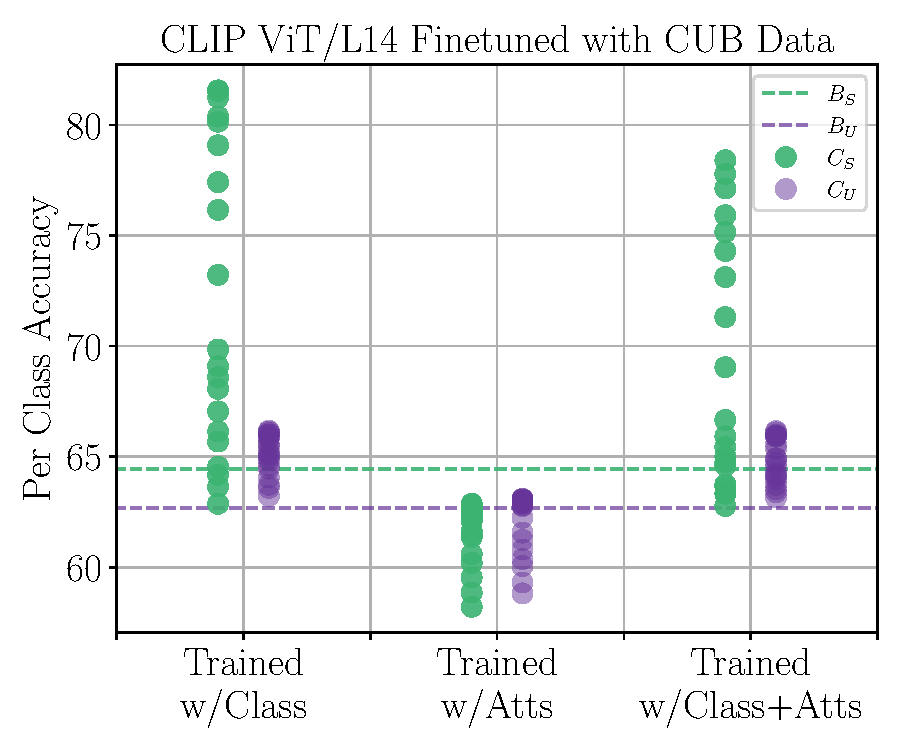
\includegraphics[width=.3\textwidth]{Images/cub_results_on_finetuned_vitl14.pdf}\hfill
\hspace{1cm}
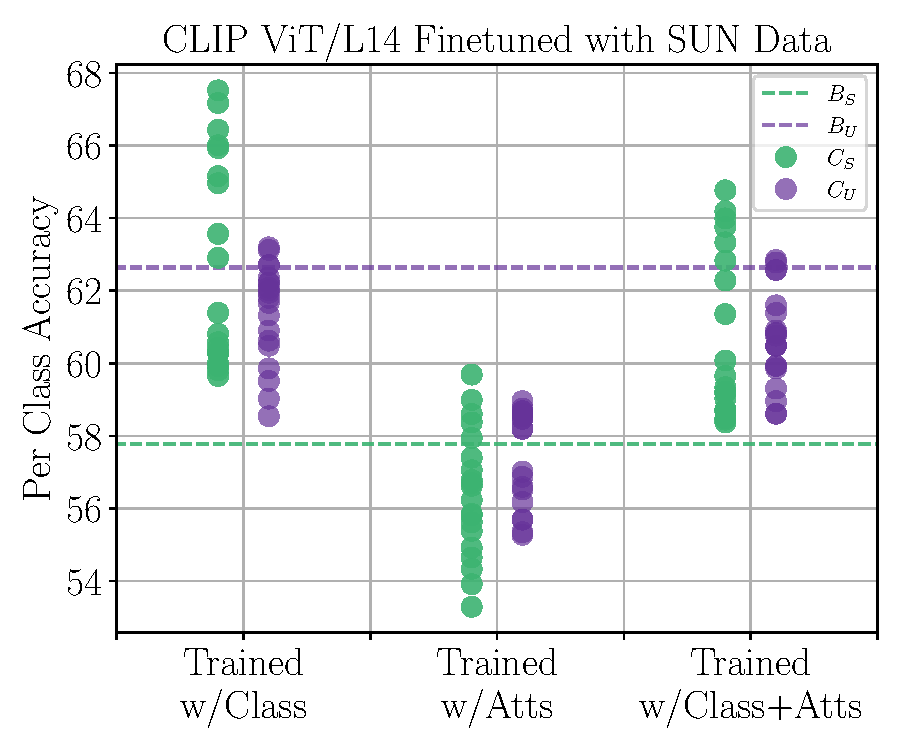
\includegraphics[width=.3\textwidth]{Images/sun_results_on_finetuned_vitl14.pdf}\hfill
\hspace{1cm}
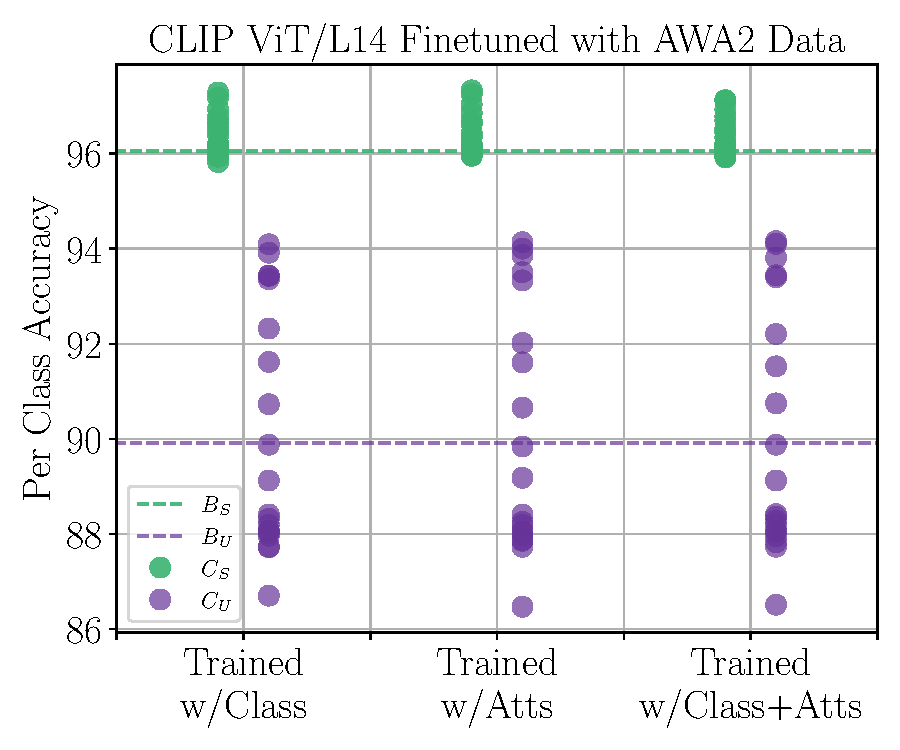
\includegraphics[width=.3\textwidth]{Images/awa2_results_on_finetuned_vitl14.pdf}
}
% \vspace{-0.2in}
\caption{\textbf{Fine-tuning CLIP with seen samples}. Results of fine-tuning a CLIP model using the images and different text descriptions, including the class name, the attribute text, and combining both text captions. We show accuracy variations after 110k training iterations for CUB\cite{CUB}, SUN\cite{SUN} and AWA2\cite{AWA2}, where B$_S$ and B$_S$ indicate the base performance of seen and unseen classes without fine-tuning. C$_S$ refers to the seen classes, and C$_U$ refers to the unseen (novel) classes after fine-tuning.} 
\label{fig:finetuned_clip_accs}
\vspace{-0.1in}
\end{figure*}
%%%%%%%%%%%%%%%%%%%%%%%%%%%%%%%%%%%%%%%%%%%%%%%%%%%%%%%%%%%%



\section{Results using CLIP as a Multimodal Feature Extractor} 
\label{sec:results_multimodal}
% \vspace{-0.2in}
\textbf{Direct evaluation of CLIP} using the images and class names without any further pre-training or post-processing: we use different template captions to generate the textual descriptions (e.g., \textit{"An image of a [class name]"}) and chose to evaluate the best-performing model with the template captions proposed by OpenAI to test on Imagenet~\cite{openai_2022}.
% ~\footnote{\href{https://bit.ly/3mt7XhS}{https://bit.ly/3mt7XhS}}. 
We also evaluate a CLIP model trained with the publicly available LAION-400M dataset~\cite{LAION400M} in the publicly available visual transformer backbone (i.e.~ViTB32). We show results in Table~\ref{tab:all_datasets_clip_only}. Overall, we expected CLIP to perform well in all the selected datasets, even with CUB, whose class names are particularly specific; similar results on this dataset have been reported in concurrent work~\cite{Vogel2022VLTabooAA}. Moreover, our results show that generative-based models work on par and even outperform CLIP when using the Resnet101 fine-tuned features, indicating that there might be room for improvement. 


\textbf{Evaluation of CLIP performance after fine-tuning} using the class
names, the attribute values and a combination of class names
$\&$ attribute values: Figure~\ref{fig:finetuned_clip_accs} shows the accuracy
variations after fine-tuning CLIP for 110k iterations using different types of text prompts, using only the seen training set for each dataset. Interestingly, we observed that fine-tuning enhances both the seen and unseen accuracy.

%%%%%%%%%%%%%%%%%%%%%%%%%%%%%%%%%%%%%%%%%%%%%%%%%%%%%%%%%%%%
\begin{figure*}[hbt!]
\centering
\scalebox{0.94}{
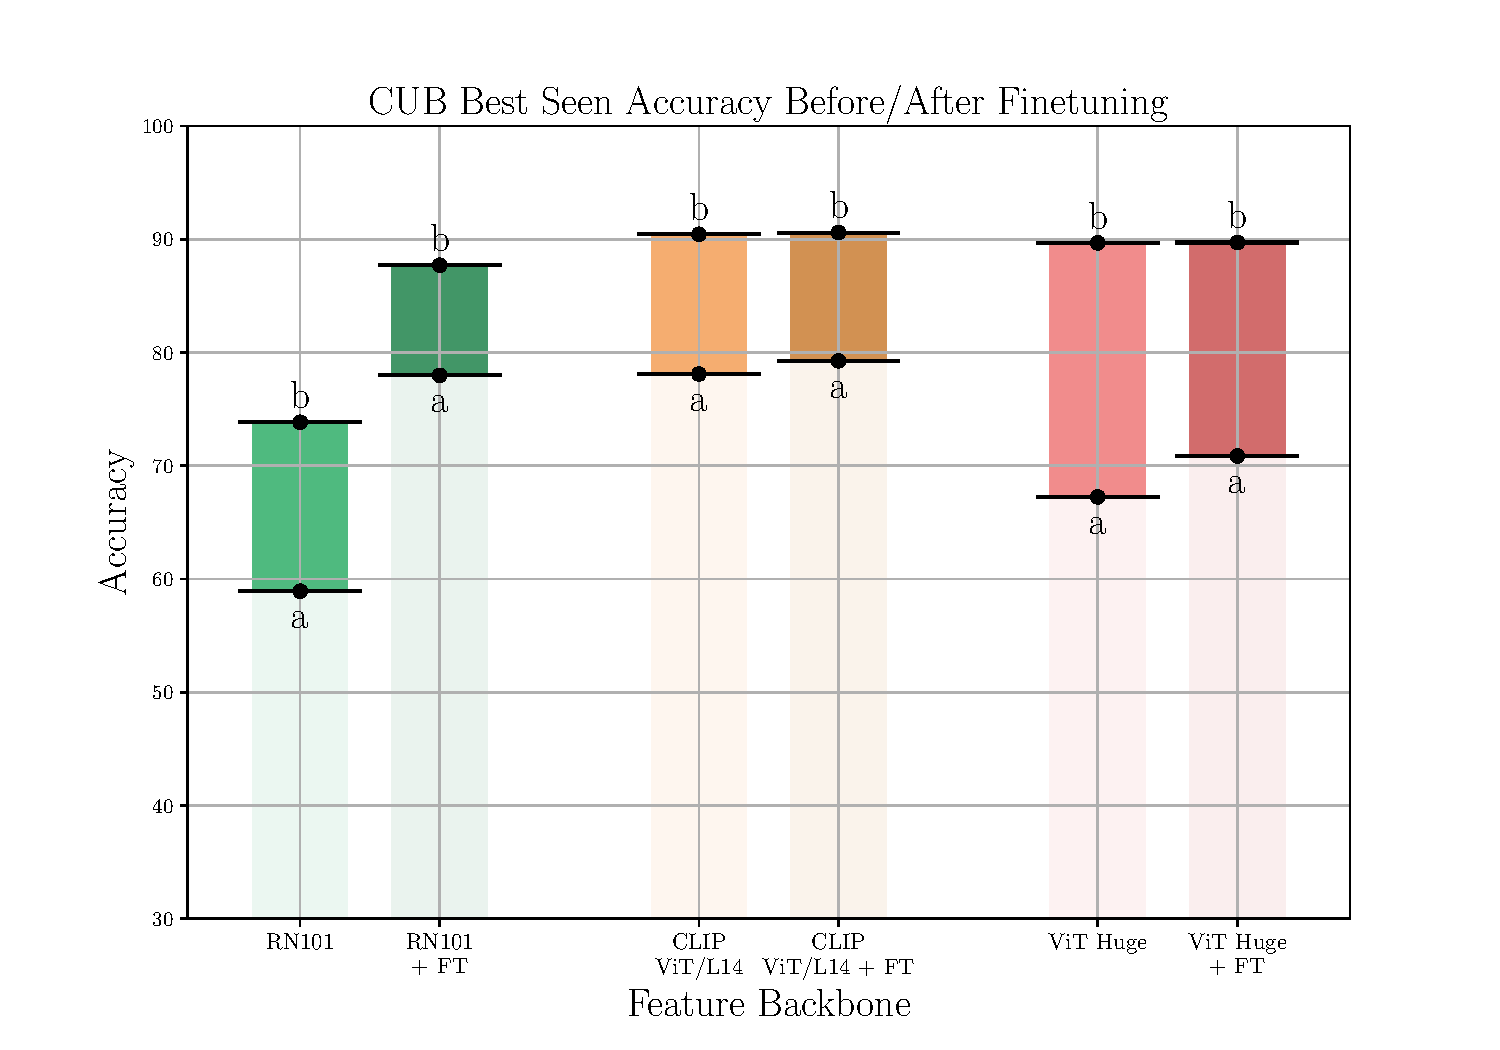
\includegraphics[width=.33\textwidth]{Images/cub_upperbound.pdf}\hfill
\hspace{0.5cm}
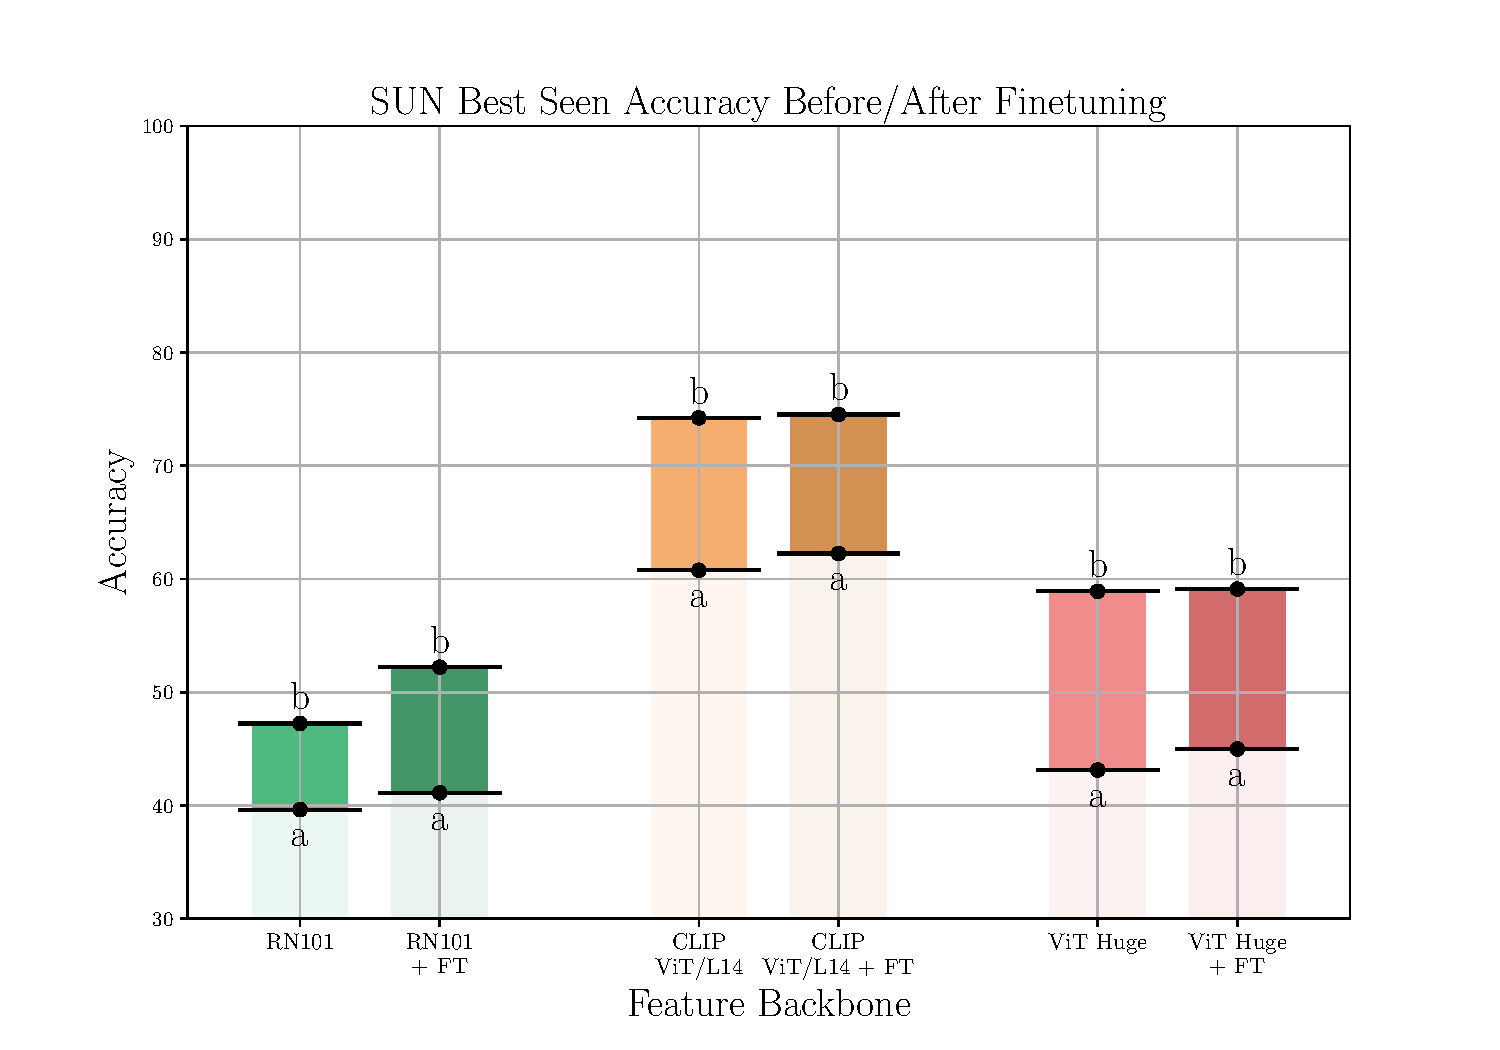
\includegraphics[width=.33\textwidth]{Images/sun_upperbound.pdf}\hfill
\hspace{0.5cm}
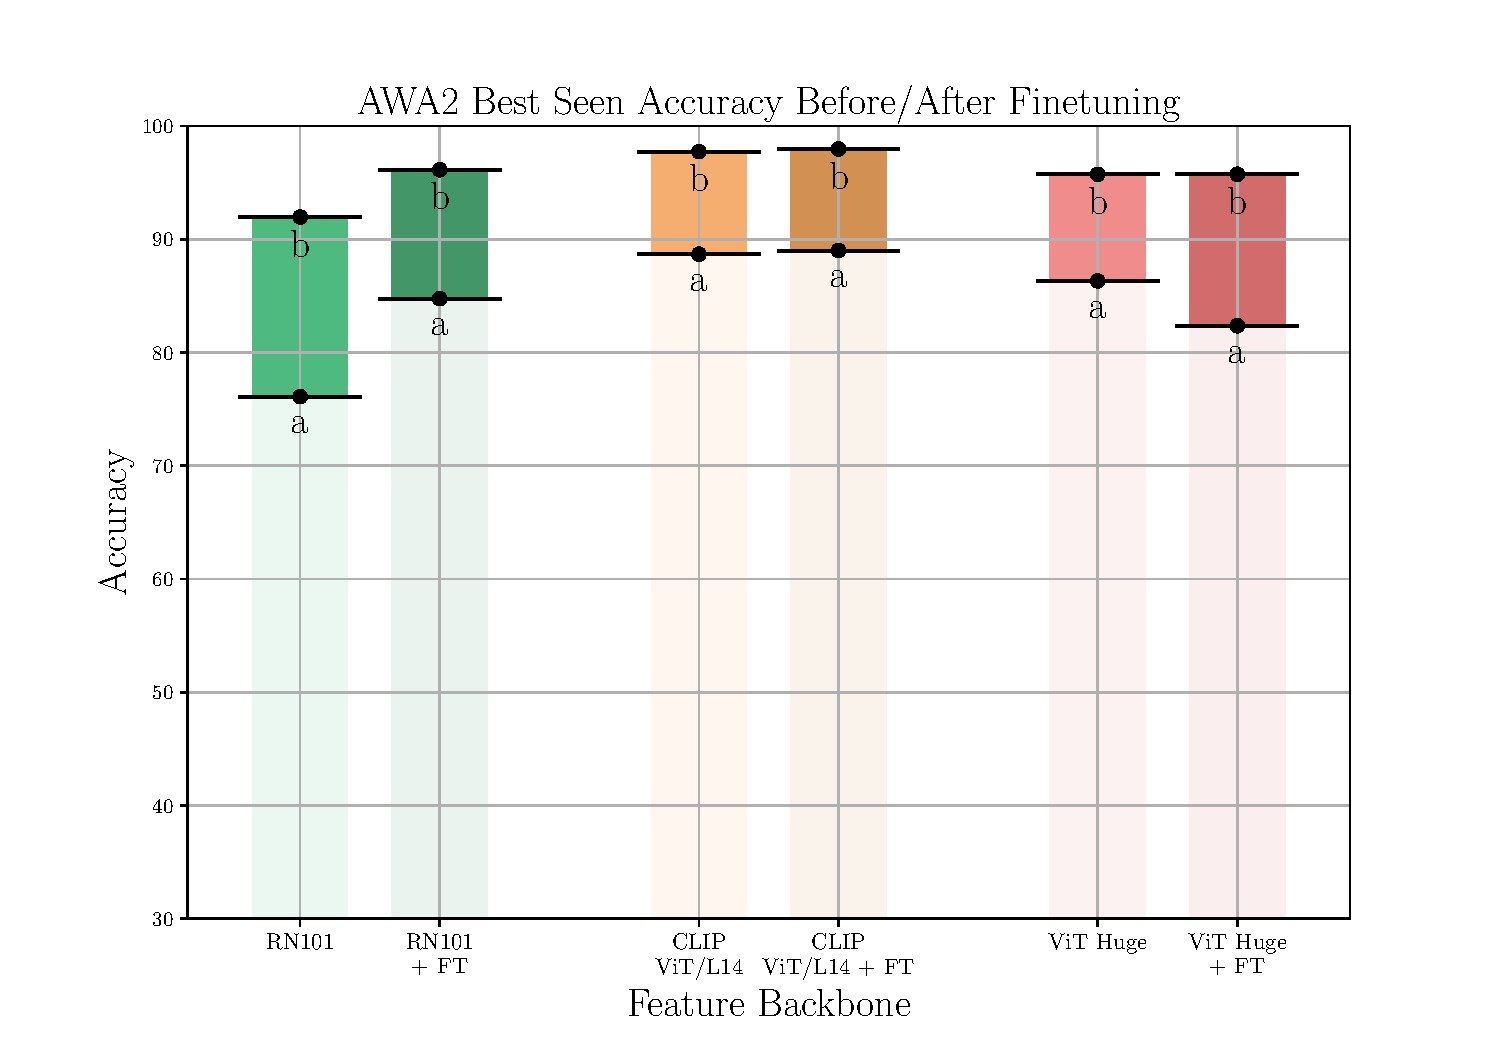
\includegraphics[width=.33\textwidth]{Images/awa2_upperbound.pdf}
}
\vspace{-0.25in}
\caption{\textbf{Fine-tuning diverse feature extractors with seen samples}. We show the difference between: a) the best-seen accuracy achieved among all GZSL methods, and b) the best-seen accuracy after training and evaluating the seen classes using a linear classifier probe. We use different visual features extracted from different backbones and training strategies. The classification upper-bound only increases significantly when fine-tuning the RN101\cite{RNs} features but remains the same with the ViT\cite{ViT} features regardless of the classification objective (i.e., cross-entropy vs. contrastive). }.
\label{fig:seen_acc_difference}
\vspace{-0.1in}
\end{figure*}

%%%%%%%%%%%%%%%%%%%%%%%%%%%%%%%%%%%%%%%%%%%%%%%%%%%%%%%%%%%%

\textbf{Evaluation of the GZSL methods using the visual features extracted from the visual encoder of CLIP}
% from (A) and (B), 
to train all GZSL methods: We show in Table~\ref{tab:gzsl_using_clip_features} the effect of using CLIP features and which fine-tuned model performs the best. Unsurprisingly, using both class name and class attributes outperforms other backbones. Similarly to uni-modal backbones, the generative-based models (e.g., CADA-VAE and tfVAEGAN) outperform other methods on all datasets. More surprisingly, both methods also outperform the CLIP results in CUB and SUN, but CLIP alone outperforms all methods in the AWA2 dataset. 
We run experiments using all eight visual encoders available from CLIP model, but show the most relevant results in Table~\ref{tab:gzsl_using_clip_features}. Please refer to the Appendix to check the full list of results.




\section{Fine-tuning Feature Extractors}


 
We observe that in the generative and disentanglement-based methods, there seems to be a trade-off in the multi-modal latent space, where some features from the seen set are distilled to the projected features of the unseen set. Typically, these methods augment the training set and convert the problem into a classification task, thus, the final seen accuracy is penalized by the classifier. 
For this reason, we also investigate how much these models penalize the final accuracy of the seen sets by measuring the difference of a classifier trained only using the seen set versus the best-seen accuracy achieved among all GZSL generative and disentanglement-based methods. 
The results are shown in Figure~\ref{fig:seen_acc_difference}. 
We observe that while fine-tuning a Resnet101 model increment the seen accuracy of both the classifier and the GZSL method, it does not increase the seen accuracy of recent models such as vision transformers. 
% Also, the improvement of the seen accuracy of the GZSL result does not improve substantially as it does with the Resnet101.
We also observe that the seen accuracy of the GZSL method does not improve substantially when using ViT features, 
% More surprisingly, 
and fine-tuning on AWA2 hurts the best seen accuracy on the GZSL result while not improving the classifier seen accuracy. 


